\documentclass[11pt]{article}

\usepackage[utf8]{inputenc}

\usepackage[T1]{fontenc}

\usepackage{graphicx}

\usepackage[margin=1in]{geometry}

\title{Phase 2: Probability and distributions -- NACC}

\author{Mahdi Aroun}

\date{phase-2}

\begin{document}

\maketitle

\section*{Task coverage}

\begin{tabular}{p{0.13\linewidth}p{0.14\linewidth}p{0.29\linewidth}p{0.29\linewidth}}

\textbf{Task} & \textbf{Status} & \textbf{Notebook} & \textbf{Report} \\

\hline

Shared 1 & Addressed & Shared Task 1 & Shared Task 1 \\

Shared 2 & Addressed & Shared Task 2 & Shared Task 2 \\

Shared 3 & Addressed & Shared Task 3 & Shared Task 3 \\

Shared 4 & Addressed & Shared Task 4 & Shared Task 4 \\

Shared 5 & Addressed & Shared Task 5 & Shared Task 5 \\

Shared 6 & Addressed & Shared Task 6 & Shared Task 6 \\

Shared 7 & Addressed & Shared Task 7 & Shared Task 7 \\

Shared 8 & Addressed & Shared Task 8 & Shared Task 8 \\

Shared 9 & Addressed & Shared Task 9 & Shared Task 9 \\

C1 & Addressed & C1 & Path C Task C1 \\

C2 & Addressed & C2 & Path C Task C2 \\

C3 & Addressed & C3 & Path C Task C3 \\

C4 & Addressed & C4 & Path C Task C4 \\

C5 & Addressed & C5 & Path C Task C5 \\

\end{tabular}

\section*{Study and participant-level frame}

Phase 2, Path C. Question: how do recorded NACCAPOE categories relate to recorded cognitive status, and how do left and right entorhinal thickness relate to CDRSUM? These are empirical descriptions, not causal effects or population estimates. Source: supplied udslong\_imputed.csv and mriscanclean.csv. UDS is already imputed; no new imputation was performed. The supplied NACC codebook was absent; no biological interpretation is assigned to NACCAPOE categories, including code 9.

\section*{Data quality and eligible outcomes}

Missing counts after joining for the six core variables: NACCAPOE: 0 (0.0\%), CDRGLOB: 0 (0.0\%), CDRSUM: 0 (0.0\%), MOCATOTS: 0 (0.0\%), LH\_ENTORHINAL\_AVGTH: 0 (0.0\%), RH\_ENTORHINAL\_AVGTH: 0 (0.0\%). Zero blank cells do not imply original complete data because the UDS input was imputed. MOCATOTS has 88, other values above 30, and fractional values; without codebook and imputation metadata we cannot interpret or clean these, so use CDRSUM rather than assume they are valid scores. CDRGLOB > 0 is a recorded-value event, not a new diagnosis. Units and clinical cutoffs are not asserted without supplied documentation.

\section*{Shared Task 1: Sample space and random variables}

Choose a participant uniformly from the 1237 eligible matched rows. A = recorded CDRGLOB > 0; B = left thickness strictly below the observed median 3.021; X = recorded CDRSUM. A and B are binary indicators of the selected participant; X is the participant's quantitative recorded clinical score and left thickness is a continuous-valued MRI measure. These choices support the probability table and paired cognitive-imaging description. Ties at the median belong to not-B.

\section*{Shared Task 2: Marginal probabilities}

A: 437/1237 = 0.3533; B: 615/1237 = 0.4972; joint A and B: 284/1237 = 0.2296.

\section*{Shared Task 3: Joint and conditional probabilities}

P(A|B) = 284/615 = 0.4618; P(A|not B) = 153/622 = 0.2460. The groups differ descriptively.

\section*{Shared Task 4: Empirical independence}

Under empirical independence P(A)P(B) = 0.1756, unlike joint 0.2296; exact independence is not compatible with these empirical proportions, without a formal test or inference.

\section*{Shared Task 5: Discrete distribution}

A is Bernoulli in the empirical distribution with p = 0.3533. For a hypothetical count K in 10 independent, identically distributed draws with replacement, K \textasciitilde{} Binomial(10,p); P(K >= 4) = 0.4951, E(K)=10p=3.533, Var(K)=10p(1-p)=2.285. This is a probability model, not resampling or a confidence interval. For 10 distinct participants sampled without replacement the exact finite-population count is hypergeometric, not binomial; similar probabilities require a small sampling fraction and comparable independent draws. Selection, center effects and repeated histories may also undermine independence or equal probabilities.

\begin{figure}[htbp]\centering

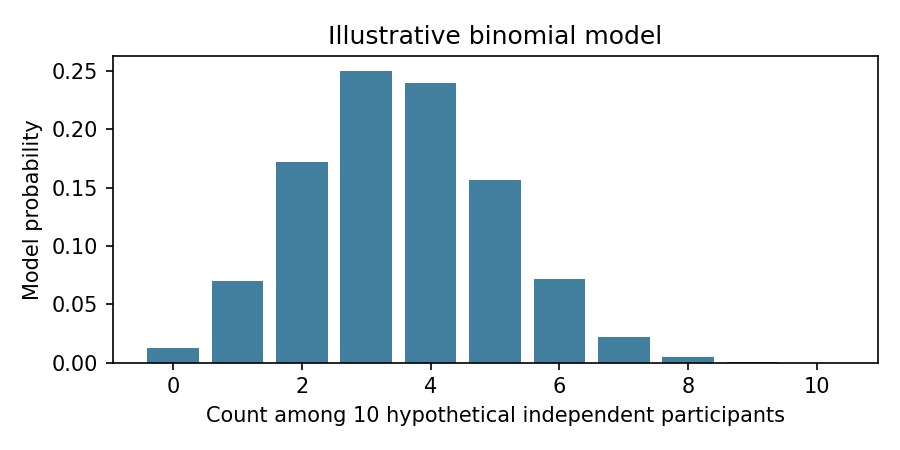
\includegraphics[width=.88\linewidth]{../../figures/binomial.png}

\caption{Illustrative model probabilities, not observed group counts.}

\end{figure}

\section*{Shared Task 6: Continuous distribution and normal approximation}

CDRSUM is strongly concentrated at zero and right-skewed, so a normal approximation is poor. Left thickness has a roughly central mound but a lower tail and deviations in the Q-Q plot; a normal model is at best approximate, especially in the tails. See the histogram and normal Q-Q plot below; the reference line uses the empirical mean and standard deviation.

\begin{figure}[htbp]\centering

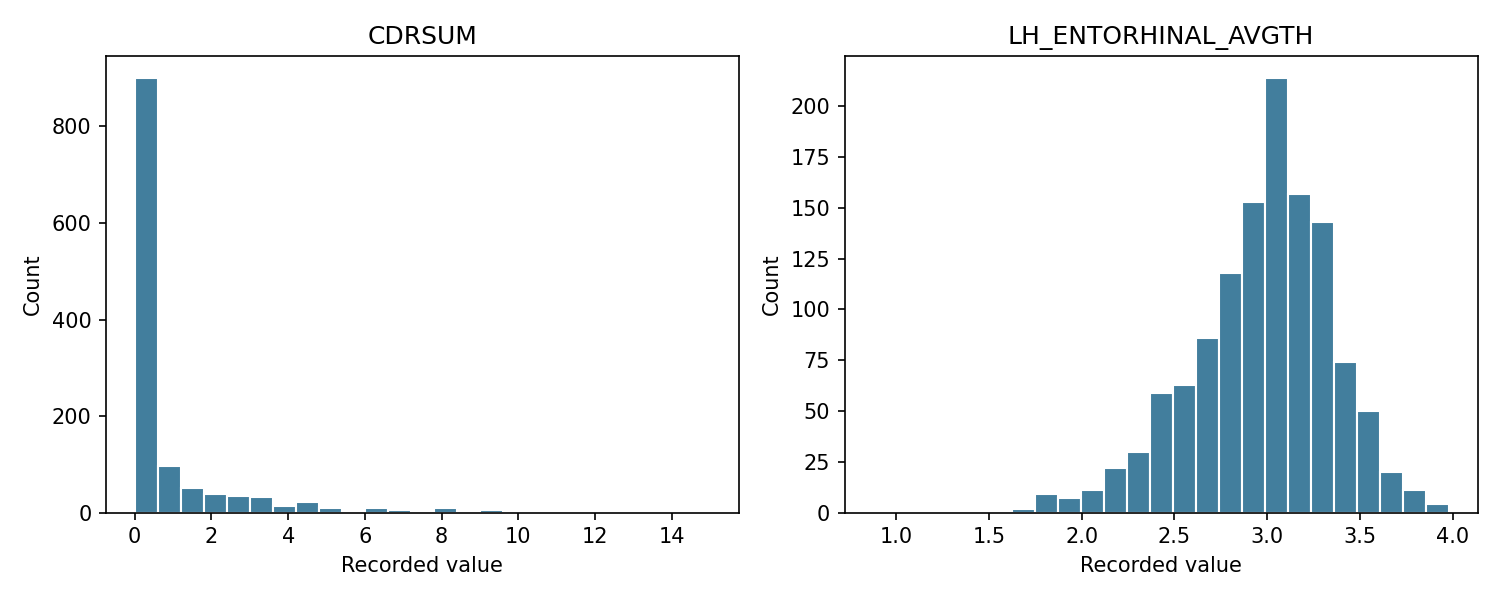
\includegraphics[width=.88\linewidth]{../../figures/distributions.png}

\caption{Observed cognitive and imaging distributions.}

\end{figure}

\begin{figure}[htbp]\centering

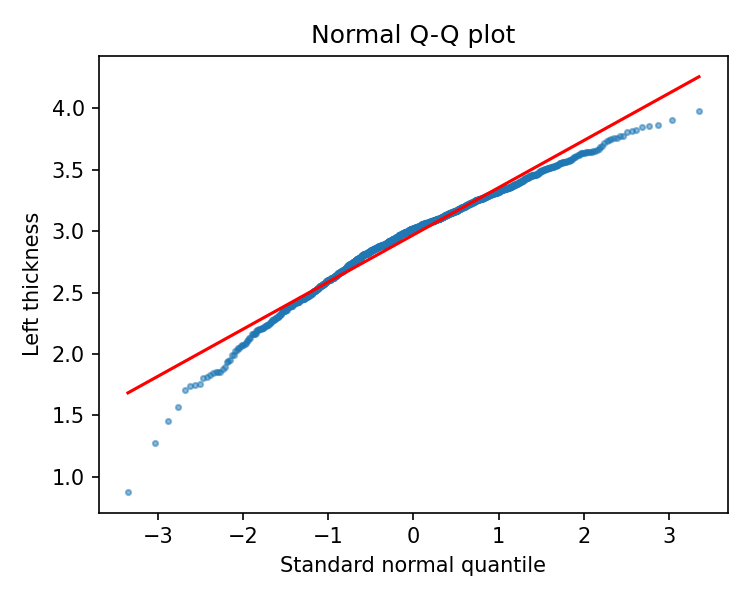
\includegraphics[width=.88\linewidth]{../../figures/qq.png}

\caption{Left thickness normal Q-Q plot and fitted mean/SD reference line.}

\end{figure}

\section*{Shared Task 7: Empirical expectation and variance}

Moments use denominator n (the empirical probability distribution); outliers are counts outside Q1 - 1.5 IQR and Q3 + 1.5 IQR, not errors to delete. CDRSUM: n=1237, mean=0.822, variance=2.966, median=0.000, range 0.000 to 15.000, Tukey flags=115. LH\_ENTORHINAL\_AVGTH: n=1237, mean=2.970, variance=0.147, median=3.021, range 0.878 to 3.979, Tukey flags=28. RH\_ENTORHINAL\_AVGTH: n=1237, mean=3.058, variance=0.161, median=3.097, range 0.729 to 3.967, Tukey flags=30. The variance describes squared dispersion around the empirical mean, not uncertainty in that mean.

\section*{Shared Task 8: Covariance}

Population-form empirical covariance uses 1/n on available pairs: cov(left thickness, CDRSUM) = -0.1775; cov(right thickness, CDRSUM) = -0.1802. Both paired denominators are 1237 (left) and 1237 (right). Negative signs indicate that larger thickness values tend to co-occur with lower CDRSUM within this file; the scatter is heterogeneous and covariance depends on measurement scales. No correlation, significance test, regression or causal conclusion is made.

\begin{figure}[htbp]\centering

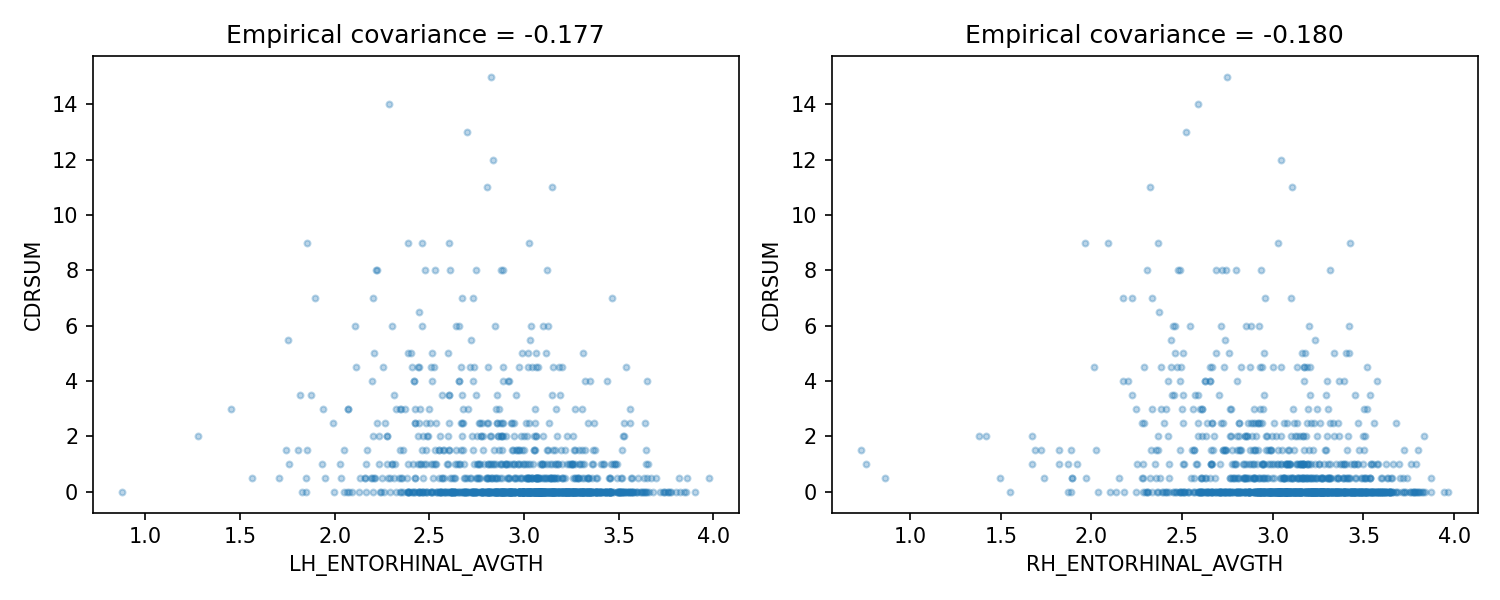
\includegraphics[width=.88\linewidth]{../../figures/scatter.png}

\caption{Bilateral thickness and recorded CDRSUM; one point per participant.}

\end{figure}

\section*{Shared Task 9: Bayes identity}

Treat B as the observed information and A as the event of interest. P(B|A) = 284/437 = 0.6499; P(A|B) = P(B|A) P(A) / P(B) = 0.4618. This is a rearrangement of the same observed table, not a validated diagnostic test, external prior, or temporal prediction.

\section*{Path C Task C1: Cognitive status in MRI and NACCAPOE groups}

The MRI grouping compares below-median versus at-or-above-median left thickness; counts, denominators and conditional probabilities appear above. The second grouping uses recorded NACCAPOE categories below. Both use the same eligible sample; differences are descriptive, not causal or tests. For each recorded code, count A / group size (proportion): 1: 129/493 (0.262); 2: 115/290 (0.397); 3: 23/83 (0.277); 4: 44/73 (0.603); 5: 4/17 (0.235); 6: 0/3 (0.000); 9: 122/278 (0.439). Code 9 is included as a raw recorded category, not assumed to be a genotype; small groups are unstable descriptions. These are not e4 carrier comparisons.

\section*{Path C Task C2: Clinical and MRI distributions}

The numeric summaries and Tukey flags are reported in Shared Task 7; histograms and shape discussion appear in Shared Task 6. These describe the supplied eligible sample.

\section*{Path C Task C3: Clinical and imaging events}

The cross-modal joint and conditional probabilities are given in Shared Tasks 2 and 3; the MRI threshold is the sample median, not a clinical cutoff. The comparison is descriptive and does not establish temporal order.

\section*{Path C Task C4: Bilateral covariance}

The complete-pair covariance values and bilateral scatterplots are reported in Shared Task 8. These are scale-dependent descriptive summaries, not causal effects.

\section*{Path C Task C5: IDs, matching and observation rule}

UDS: 1237 rows and 1237 unique nonmissing IDs; MRI: 1237 rows and 1237 unique IDs. UDS-only 0, MRI-only 0, one-to-one matched 1237. Analysis includes 1237 rows with nonmissing left thickness and CDRGLOB in observed values 0, 0.5, 1, 2. Each participant contributes the only supplied row; no index visit can be selected chronologically. A unique row is not evidence of independence between people, a single historical visit, or contemporaneous UDS and MRI. No reliable visit/scan timing is supplied; historical visit counts and lag are unknown.

\section*{Limitations and next steps}

MRI inclusion cannot be compared with non-MRI participants because all supplied UDS IDs match MRI. Selection into the supplied cohort is unknown. Imputed and special values may influence results; codebook and original missingness are unavailable. Obtain authoritative coding and visit/scan timing before interpreting genotype or clinical status, and before later inference. The median cutoff is sample-defined, not clinical. No Phase 3-5 analyses were performed.

\end{document}